%% bare_conf.tex
%% V1.3
%% 2007/01/11
%% by Michael Shell
%% See:
%% http://www.michaelshell.org/
%% for current contact information.
%%
%% This is a skeleton file demonstrating the use of IEEEtran.cls
%% (requires IEEEtran.cls version 1.7 or later) with an IEEE conference paper.
%%
%% Support sites:
%% http://www.michaelshell.org/tex/ieeetran/
%% http://www.ctan.org/tex-archive/macros/latex/contrib/IEEEtran/
%% and
%% http://www.ieee.org/

%%*************************************************************************
%% Legal Notice:
%% This code is offered as-is without any warranty either expressed or
%% implied; without even the implied warranty of MERCHANTABILITY or
%% FITNESS FOR A PARTICULAR PURPOSE!

%% User assumes all risk.
%% In no event shall IEEE or any contributor to this code be liable for
%% any damages or losses, including, but not limited to, incidental,
%% consequential, or any other damages, resulting from the use or misuse
%% of any information contained here.
%%
%% All comments are the opinions of their respective authors and are not
%% necessarily endorsed by the IEEE.
%%
%% This work is distributed under the LaTeX Project Public License (LPPL)
%% ( http://www.latex-project.org/ ) version 1.3, and may be freely used,
%% distributed and modified. A copy of the LPPL, version 1.3, is included
%% in the base LaTeX documentation of all distributions of LaTeX released
%% 2003/12/01 or later.
%% Retain all contribution notices and credits.
%% ** Modified files should be clearly indicated as such, including  **
%% ** renaming them and changing author support contact information. **
%%
%% File list of work: IEEEtran.cls, IEEEtran_HOWTO.pdf, bare_adv.tex,
%%                    bare_conf.tex, bare_jrnl.tex, bare_jrnl_compsoc.tex
%%*************************************************************************

% *** Authors should verify (and, if needed, correct) their LaTeX system  ***
% *** with the testflow diagnostic prior to trusting their LaTeX platform ***
% *** with production work. IEEE's font choices can trigger bugs that do  ***
% *** not appear when using other class files.                            ***
% The testflow support page is at:
% http://www.michaelshell.org/tex/testflow/



% Note that the a4paper option is mainly intended so that authors in
% countries using A4 can easily print to A4 and see how their papers will
% look in print - the typesetting of the document will not typically be
% affected with changes in paper size (but the bottom and side margins will).
% Use the testflow package mentioned above to verify correct handling of
% both paper sizes by the user's LaTeX system.
%
% Also note that the "draftcls" or "draftclsnofoot", not "draft", option
% should be used if it is desired that the figures are to be displayed in
% draft mode.
%
\documentclass[conference]{IEEEtran}
% Add the compsoc option for Computer Society conferences.
%
% If IEEEtran.cls has not been installed into the LaTeX system files,
% manually specify the path to it like:
% \documentclass[conference]{../sty/IEEEtran}





% Some very useful LaTeX packages include:
% (uncomment the ones you want to load)


% *** MISC UTILITY PACKAGES ***
%
%\usepackage{ifpdf}
% Heiko Oberdiek's ifpdf.sty is very useful if you need conditional
% compilation based on whether the output is pdf or dvi.
% usage:
% \ifpdf
%   % pdf code
% \else
%   % dvi code
% \fi
% The latest version of ifpdf.sty can be obtained from:
% http://www.ctan.org/tex-archive/macros/latex/contrib/oberdiek/
% Also, note that IEEEtran.cls V1.7 and later provides a builtin
% \ifCLASSINFOpdf conditional that works the same way.
% When switching from latex to pdflatex and vice-versa, the compiler may
% have to be run twice to clear warning/error messages.

%\usepackage{geometry}
%\geometry{left=2.5cm,right=2.5cm,top=2.5cm,bottom=2.5cm}




% *** CITATION PACKAGES ***
%
\usepackage{cite}
% cite.sty was written by Donald Arseneau
% V1.6 and later of IEEEtran pre-defines the format of the cite.sty package
% \cite{} output to follow that of IEEE. Loading the cite package will
% result in citation numbers being automatically sorted and properly
% "compressed/ranged". e.g., [1], [9], [2], [7], [5], [6] without using
% cite.sty will become [1], [2], [5]--[7], [9] using cite.sty. cite.sty's
% \cite will automatically add leading space, if needed. Use cite.sty's
% noadjust option (cite.sty V3.8 and later) if you want to turn this off.
% cite.sty is already installed on most LaTeX systems. Be sure and use
% version 4.0 (2003-05-27) and later if using hyperref.sty. cite.sty does
% not currently provide for hyperlinked citations.
% The latest version can be obtained at:
% http://www.ctan.org/tex-archive/macros/latex/contrib/cite/
% The documentation is contained in the cite.sty file itself.

\usepackage[normalem]{ulem}
\newcommand{\rev}[1]{\uwave{#1}}  %revise the text


\newcommand{\del}[1]{\sout{#1}}  %revise the text

%\newcommand{\del}[1]{}

\newcommand{\note}[1]{{\sffamily\itshape\bfseries\uline{#1}}}
\usepackage{multirow}
\usepackage{graphicx}
\usepackage{subfigure}
\usepackage{bm}
\usepackage{amsfonts}
\usepackage{url}
% *** GRAPHICS RELATED PACKAGES ***
%
\ifCLASSINFOpdf
  % \usepackage[pdftex]{graphicx}
  % declare the path(s) where your graphic files are
  
  %%%%modifiesd by jj
   \graphicspath{{./graph/}}
   
  % and their extensions so you won't have to specify these with
  % every instance of \includegraphics
  % \DeclareGraphicsExtensions{.pdf,.jpeg,.png}
\else
  % or other class option (dvipsone, dvipdf, if not using dvips). graphicx
  % will default to the driver specified in the system graphics.cfg if no
  % driver is specified.
  % \usepackage[dvips]{graphicx}
  % declare the path(s) where your graphic files are
  % \graphicspath{{../eps/}}
  % and their extensions so you won't have to specify these with
  % every instance of \includegraphics
  % \DeclareGraphicsExtensions{.eps}
\fi
% graphicx was written by David Carlisle and Sebastian Rahtz. It is
% required if you want graphics, photos, etc. graphicx.sty is already
% installed on most LaTeX systems. The latest version and documentation can
% be obtained at:
% http://www.ctan.org/tex-archive/macros/latex/required/graphics/
% Another good source of documentation is "Using Imported Graphics in
% LaTeX2e" by Keith Reckdahl which can be found as epslatex.ps or
% epslatex.pdf at: http://www.ctan.org/tex-archive/info/
%
% latex, and pdflatex in dvi mode, support graphics in encapsulated
% postscript (.eps) format. pdflatex in pdf mode supports graphics
% in .pdf, .jpeg, .png and .mps (metapost) formats. Users should ensure
% that all non-photo figures use a vector format (.eps, .pdf, .mps) and
% not a bitmapped formats (.jpeg, .png). IEEE frowns on bitmapped formats
% which can result in "jaggedy"/blurry rendering of lines and letters as
% well as large increases in file sizes.
%
% You can find documentation about the pdfTeX application at:
% http://www.tug.org/applications/pdftex

\usepackage{graphicx}



% *** MATH PACKAGES ***
%
\usepackage[cmex10]{amsmath}
% A popular package from the American Mathematical Society that provides
% many useful and powerful commands for dealing with mathematics. If using
% it, be sure to load this package with the cmex10 option to ensure that
% only type 1 fonts will utilized at all point sizes. Without this option,
% it is possible that some math symbols, particularly those within
% footnotes, will be rendered in bitmap form which will result in a
% document that can not be IEEE Xplore compliant!
%
% Also, note that the amsmath package sets \interdisplaylinepenalty to 10000
% thus preventing page breaks from occurring within multiline equations. Use:
%\interdisplaylinepenalty=2500
% after loading amsmath to restore such page breaks as IEEEtran.cls normally
% does. amsmath.sty is already installed on most LaTeX systems. The latest
% version and documentation can be obtained at:
% http://www.ctan.org/tex-archive/macros/latex/required/amslatex/math/





% *** SPECIALIZED LIST PACKAGES ***
%
\usepackage{algorithmic}



% algorithmic.sty was written by Peter Williams and Rogerio Brito.
% This package provides an algorithmic environment fo describing algorithms.
% You can use the algorithmic environment in-text or within a figure
% environment to provide for a floating algorithm. Do NOT use the algorithm
% floating environment provided by algorithm.sty (by the same authors) or
% algorithm2e.sty (by Christophe Fiorio) as IEEE does not use dedicated
% algorithm float types and packages that provide these will not provide
% correct IEEE style captions. The latest version and documentation of
% algorithmic.sty can be obtained at:
% http://www.ctan.org/tex-archive/macros/latex/contrib/algorithms/
% There is also a support site at:
% http://algorithms.berlios.de/index.html
% Also of interest may be the (relatively newer and more customizable)
% algorithmicx.sty package by Szasz Janos:
% http://www.ctan.org/tex-archive/macros/latex/contrib/algorithmicx/
%\usepackage{algorithm}
\usepackage[]{algorithm2e}
\makeatletter
\renewcommand{\@algocf@capt@plain}{above}% formerly {bottom}
\makeatother

\usepackage{amsthm}

\usepackage[table,xcdraw]{xcolor}

% *** ALIGNMENT PACKAGES ***
%
%\usepackage{array}
% Frank Mittelbach's and David Carlisle's array.sty patches and improves
% the standard LaTeX2e array and tabular environments to provide better
% appearance and additional user controls. As the default LaTeX2e table
% generation code is lacking to the point of almost being broken with
% respect to the quality of the end results, all users are strongly
% advised to use an enhanced (at the very least that provided by array.sty)
% set of table tools. array.sty is already installed on most systems. The
% latest version and documentation can be obtained at:
% http://www.ctan.org/tex-archive/macros/latex/required/tools/


%\usepackage{mdwmath}
%\usepackage{mdwtab}
% Also highly recommended is Mark Wooding's extremely powerful MDW tools,
% especially mdwmath.sty and mdwtab.sty which are used to format equations
% and tables, respectively. The MDWtools set is already installed on most
% LaTeX systems. The lastest version and documentation is available at:
% http://www.ctan.org/tex-archive/macros/latex/contrib/mdwtools/


% IEEEtran contains the IEEEeqnarray family of commands that can be used to
% generate multiline equations as well as matrices, tables, etc., of high
% quality.


%\usepackage{eqparbox}
% Also of notable interest is Scott Pakin's eqparbox package for creating
% (automatically sized) equal width boxes - aka "natural width parboxes".
% Available at:
% http://www.ctan.org/tex-archive/macros/latex/contrib/eqparbox/





% *** SUBFIGURE PACKAGES ***
%\usepackage[tight,footnotesize]{subfigure}
% subfigure.sty was written by Steven Douglas Cochran. This package makes it
% easy to put subfigures in your figures. e.g., "Figure 1a and 1b". For IEEE
% work, it is a good idea to load it with the tight package option to reduce
% the amount of white space around the subfigures. subfigure.sty is already
% installed on most LaTeX systems. The latest version and documentation can
% be obtained at:
% http://www.ctan.org/tex-archive/obsolete/macros/latex/contrib/subfigure/
% subfigure.sty has been superceeded by subfig.sty.



%\usepackage[caption=false]{caption}
%\usepackage[font=footnotesize]{subfig}
% subfig.sty, also written by Steven Douglas Cochran, is the modern
% replacement for subfigure.sty. However, subfig.sty requires and
% automatically loads Axel Sommerfeldt's caption.sty which will override
% IEEEtran.cls handling of captions and this will result in nonIEEE style
% figure/table captions. To prevent this problem, be sure and preload
% caption.sty with its "caption=false" package option. This is will preserve
% IEEEtran.cls handing of captions. Version 1.3 (2005/06/28) and later
% (recommended due to many improvements over 1.2) of subfig.sty supports
% the caption=false option directly:
%\usepackage[caption=false,font=footnotesize]{subfig}
%
% The latest version and documentation can be obtained at:
% http://www.ctan.org/tex-archive/macros/latex/contrib/subfig/
% The latest version and documentation of caption.sty can be obtained at:
% http://www.ctan.org/tex-archive/macros/latex/contrib/caption/




% *** FLOAT PACKAGES ***
%
%\usepackage{fixltx2e}
% fixltx2e, the successor to the earlier fix2col.sty, was written by
% Frank Mittelbach and David Carlisle. This package corrects a few problems
% in the LaTeX2e kernel, the most notable of which is that in current
% LaTeX2e releases, the ordering of single and double column floats is not
% guaranteed to be preserved. Thus, an unpatched LaTeX2e can allow a
% single column figure to be placed prior to an earlier double column
% figure. The latest version and documentation can be found at:
% http://www.ctan.org/tex-archive/macros/latex/base/



%\usepackage{stfloats}
% stfloats.sty was written by Sigitas Tolusis. This package gives LaTeX2e
% the ability to do double column floats at the bottom of the page as well
% as the top. (e.g., "\begin{figure*}[!b]" is not normally possible in
% LaTeX2e). It also provides a command:
%\fnbelowfloat
% to enable the placement of footnotes below bottom floats (the standard
% LaTeX2e kernel puts them above bottom floats). This is an invasive package
% which rewrites many portions of the LaTeX2e float routines. It may not work
% with other packages that modify the LaTeX2e float routines. The latest
% version and documentation can be obtained at:
% http://www.ctan.org/tex-archive/macros/latex/contrib/sttools/
% Documentation is contained in the stfloats.sty comments as well as in the
% presfull.pdf file. Do not use the stfloats baselinefloat ability as IEEE
% does not allow \baselineskip to stretch. Authors submitting work to the
% IEEE should note that IEEE rarely uses double column equations and
% that authors should try to avoid such use. Do not be tempted to use the
% cuted.sty or midfloat.sty packages (also by Sigitas Tolusis) as IEEE does
% not format its papers in such ways.





% *** PDF, URL AND HYPERLINK PACKAGES ***
%
%\usepackage{url}
% url.sty was written by Donald Arseneau. It provides better support for
% handling and breaking URLs. url.sty is already installed on most LaTeX
% systems. The latest version can be obtained at:
% http://www.ctan.org/tex-archive/macros/latex/contrib/misc/
% Read the url.sty source comments for usage information. Basically,
% \url{my_url_here}.





% *** Do not adjust lengths that control margins, column widths, etc. ***
% *** Do not use packages that alter fonts (such as pslatex).         ***
% There should be no need to do such things with IEEEtran.cls V1.6 and later.
% (Unless specifically asked to do so by the journal or conference you plan
% to submit to, of course. )


% correct bad hyphenation here
\hyphenation{op-tical net-works semi-conduc-tor}




\begin{document}
%
% paper title
% can use linebreaks \\ within to get better formatting as desired
\title{}

\title{Detecting the DOA for Robots with Wireless Antennas}

\author{\IEEEauthorblockN{ Xin Wang\IEEEauthorrefmark{2}, Zhe Yan\IEEEauthorrefmark{2}, Bumsik Kim\IEEEauthorrefmark{2} and Jiejie Wei\IEEEauthorrefmark{2}  }
\IEEEauthorblockA{Department of ECE,
Stony Brook University\\
NY,Stony Brook, 11790\\
Email: \IEEEauthorrefmark{3} xin.wang@stonybrook.edu, \IEEEauthorrefmark{3} zhe.yan@stonybrook.edu, 
\IEEEauthorrefmark{2} bumsik.kim@stonybrook.edu, \IEEEauthorrefmark{2}jiejie.wei@stonybrook.edu }
}
\maketitle

% author names and affiliations
% use a multiple column layout for up to three different
% affiliations
%\author
%{
%\IEEEauthorblockN{}
%\IEEEauthorblockA{Dept of ECE\\
%Stony Brook University\\
%NY, Stony Brook 11790\\
%Email: zhe.yan@stonybrook.edu}
%\and
%\IEEEauthorblockN{Hanho Lee}
%\IEEEauthorblockA{Dept of ECE\\
%%Electrical and\\Computer Engineering\\
%Stony Brook University\\
%NY, Stony Brook 11790\\
%Email: hanho.lee@stonybrook.edu}


%\and
%\IEEEauthorblockN{Xin Wang}
%\IEEEauthorblockA{Dept of ECE\\
%%Electrical and\\Computer Engineering\\
%Stony Brook University\\
%NY, Stony Brook 11790\\
%Email: xwang@ece.sunysb.edu}
%
%\and
%\IEEEauthorblockN{Daegeun Yoon}
%\IEEEauthorblockA{Dept of ECE\\
%%Electrical and\\Computer Engineering\\
%Stony Brook University\\
%NY, Stony Brook 11790\\
%Email: ykudfor1@gmail.com}

%\and
%\IEEEauthorblockN{Dongliang Xie}
%\IEEEauthorblockA{Dept of ECE\\
%%Electrical and\\Computer Engineering\\
%Beijing University of Posts and Telecommunications\\
%NY, Stony Brook 11790\\
%Email: 	Dongliangxie@gmail.com}
%}

% conference papers do not typically use \thanks and this command
% is locked out in conference mode. If really needed, such as for
% the acknowledgment of grants, issue a \IEEEoverridecommandlockouts
% after \documentclass

% for over three affiliations, or if they all won't fit within the width
% of the page, use this alternative format:
%
%\author{\IEEEauthorblockN{Michael Shell\IEEEauthorrefmark{1},
%Homer Simpson\IEEEauthorrefmark{2},
%James Kirk\IEEEauthorrefmark{3},
%Montgomery Scott\IEEEauthorrefmark{3} and
%Eldon Tyrell\IEEEauthorrefmark{4}}
%\IEEEauthorblockA{\IEEEauthorrefmark{1}School of Electrical and Computer Engineering\\
%Georgia Institute of Technology,
%Atlanta, Georgia 30332--0250\\ Email: see http://www.michaelshell.org/contact.html}
%\IEEEauthorblockA{\IEEEauthorrefmark{2}Twentieth Century Fox, Springfield, USA\\
%Email: homer@thesimpsons.com}
%\IEEEauthorblockA{\IEEEauthorrefmark{3}Starfleet Academy, San Francisco, California 96678-2391\\
%Telephone: (800) 555--1212, Fax: (888) 555--1212}
%\IEEEauthorblockA{\IEEEauthorrefmark{4}Tyrell Inc., 123 Replicant Street, Los Angeles, California 90210--4321}}




% use for special paper notices
%\IEEEspecialpapernotice{(Invited Paper)}




% make the title area
\maketitle

\begin{abstract}
The technology of robot grows everyday, which leads the need for a good design in their localization. Our project develops algorithms and protocols for the localization of sensors and mobile robots. The main problem is to find the direction and distance of the robots. We will use Multiple Signal Classification(MUSIC) algorithm to determine the direction of arrival(DOA) of robots, and we will estimate the distance between each of the robot based on the path loss of our received signal strength. Noise during the signal processing will be considered during our simulation. In our first semester of research, we are going to simulate the random location of robots and test the power received in ideal case and in the semester we will design our own algorithm to gather robots for better communication, calculate all proper parameters for localization and simulate them all in MATLAB.
\end{abstract}

\section{Introduction}
\label{sec:introduction}
\subsection{Background}
	There are many robots created to improve quality of our life, so the AI of robots can make a great contribution. What's more, we may want to easily find a specific room location even when we are not familiar with the place. We can navigate our outdoor position with GPS, but it is hard for us to know our indoor position with our smart devices. All of these problems lead to the topic on how to implement the localization of our robots.
\par
	In terms of localization, our method to find direction first and measure the distance along with the direction. There are several algorithms of direction of arrival, we choose to use MUSIC[1], stands for MUiltiple SIgnal Classification, one of
the high resolution subspace DOA algorithms, which gives the estimation of number of signals arrived, hence their direction of arrival. Compare with other algorithm, it is able to estimate frequencies with accuracy higher than one sample, because its estimation function can be evaluated for any frequency. This is a form of superresolution. MUSIC estimates the frequency content of a signal or autocorrelation matrix using an eigenspace method. This method assumes that a signal, $x(n)$, consists of $p$ complex exponentials in the presence of Gaussian white noise. Given an $M \times M$ autocorrelation matrix, $\mathbf{R}_x$, if the eigenvalues are sorted in decreasing order, the eigenvectors corresponding to the p largest eigenvalues (i.e. directions of largest variability) span the signal subspace. The remaining $M-p$ eigenvectors span the orthogonal space, where there is only noise. Note that for $M = p + 1$, MUSIC is identical to Pisarenko harmonic decomposition. The general idea is to use averaging to improve the performance of the Pisarenko estimator. The equation of MUSIC will be described later.
\par
	After the procedure of DOA, we will estimate distance based on path loss[2] with noise of Rayleigh fading and Gaussian white noise. Path loss is the reduction in power density of an electromagnetic wave as it propagates through space. This term is commonly used in wireless communications and signal propagation. Although path loss may be due to many effects, such as free-space loss, refraction, diffraction, reflection, aperture-medium coupling loss, and absorption, we decide to use simple version of pass loss equation without considering so many effects, which is commonly used and called free space propagation. The simplified equation will be described later.
\par
	In terms of noise simulation, we decide to use the effect of Rayleigh fading,a statistical model for the effect of a propagation environment on a radio signal, such as that used by wireless devices. Rayleigh fading models[3] assume that the magnitude of a signal that has passed through such a transmission medium (also called a communications channel) will vary randomly, or fade, according to a Rayleigh distribution — the radial component of the sum of two uncorrelated Gaussian random variables. Rayleigh fading is most applicable when there is no dominant propagation along a line of sight between the transmitter and receiver. In addition to Rayleigh fading noise, we also add Gaussian white noise, which is also known as normal distribution white noise. It is very commonly used in signal processing because of the central limit theorem, it states that averages of random variables independently drawn from independent distributions converge in distribution to the normal, that is, become normally distributed when the number of random variables is sufficiently large.  A random variable with a Gaussian distribution is said to be normally distributed and is called a normal deviate if mean of the distribution is 0 and its standard deviation is 1.


\subsection{Related Work}
Daniel B. Faria[4], published a report, "Modeling Signal Attenuation in IEEE 802.11 Wireless LANs", presented experimental data that validates the use of the log-distance model both inside and outside a standard office building. In his project, path loss models are used to approximate signal attenuation as a function of the distance between transmitters and receivers, being an important building block for both research and industry efforts. Based on experiments with off-the-shelf 802.11 hardware, they had shown that the log-distance path loss model with log-normal shadowing can be used to estimate signal attenuation both inside and outside an office building with moderate accuracy. As a result, we will not consider the environment effect of indoor and outdoor in our project.
\par
R.C. Smith and P. Cheeseman in 1986, and the research group of Hugh F. Durrant-Whyte in the early 1990s[5], proposed an algorithm called simultaneous localization and mapping (SLAM),which is the computational problem of constructing or updating a map of an unknown environment while simultaneously keeping track of an agent's location within it. 
\par
Leonard, J.J. and Durrant-Whyte, H.F.[6], proposed a report of mobile robot localization by tracking geometric beacons in 1991. The algorithm is based on an extended Kalman filter that utilizes matches between observed geometric beacons and an a priori map of beacon locations. Two implementations of this navigation algorithm, both of which use sonar, are described. The first implementation uses a simple vehicle with point kinematics equipped with a single rotating sonar. The second implementation uses a `Robuter' mobile robot and six static sonar transducers to provide localization information while the vehicle moves at typical speeds of 30 cm/s.
%\begin{figure}[h]
%\centering
%\includegraphics[width=0.8\linewidth]{img/img1}
%\caption{3D terrain surface}
%\label{fig4}
%\end{figure} 

%application \cite{Sichitiu, Musolesi2009}
%realistic \cite{Jardosh2003}
%general survey \cite{Camp2002,Bai2004}
%group \cite{Hong1999}
%probability \cite{Mohimani2009}


\section{Overview}
\label{sec:overview}
	
	\begin{figure}[ht]
	\centering
	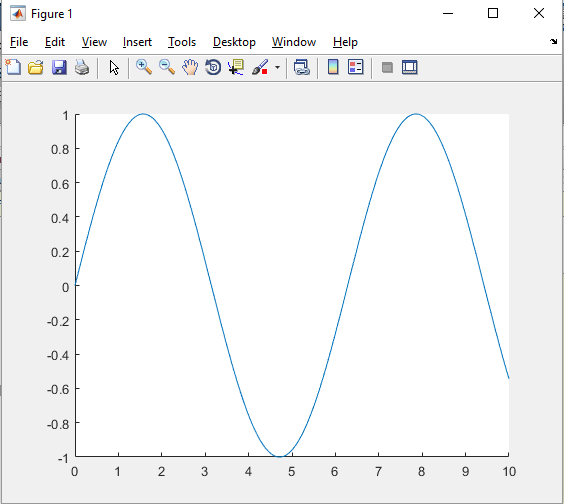
\includegraphics[width=0.4\textwidth]{noise1}
	\caption{sin waveform}
	%\label{fig1}
	\end{figure}
	
	\begin{figure}[ht]
	\centering
	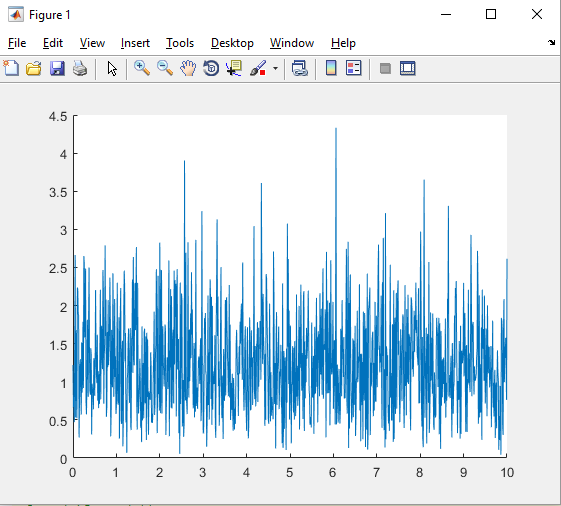
\includegraphics[width=0.4\textwidth]{noise2}
	\caption{Rayleigh fading noise}
	%\label{fig1}
	\end{figure}

	\begin{figure}[ht]
	\centering
	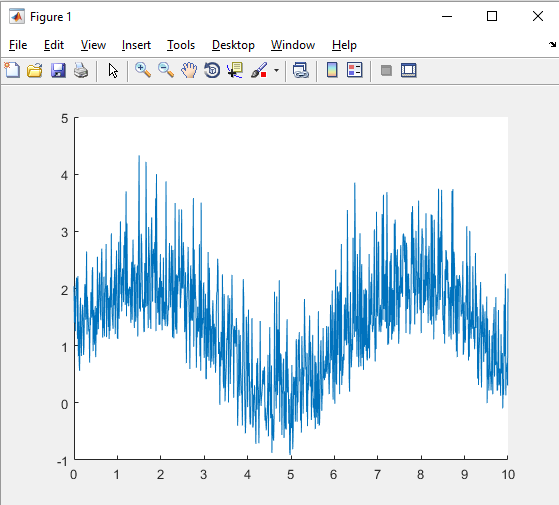
\includegraphics[width=0.4\textwidth]{noise3}
	\caption{sin waveform added with Rayleigh fading noise}
	%\label{fig1}
	\end{figure}
	
	Signal will fade during the transmitting and power will somewhat loss no matter what kind of transmitter be used. As a result, we can estimate the distance between the receiver and transmitter if we know the properties of the wireless signal. Meanwhile, the phase of signal will shift when receiver get a signal, which related to their direction of arrival. In this case, out project decide to use the MUSIC algorithm and path loss to estimate direction and distance between multiple robots.
	\par
	Due to the interaction of noise, one of the biggest challenge is to recover the original signal with considering white noise and Rayleigh fading noise. To easily understand the effect of these noise, the following figures are the simulation of some common signals when addictive noise is applied.
	
	\par
	To simulate our signal processing, we are going to use Matlab to model signals and apply them in simulation field, then we will integrate them with MUSIC algorithm and finally get DOA location, which will be described in detail later. 

%\begin{figure}[h]
%\centering
%\includegraphics[width=1.0\linewidth]{img/structure}
%\caption{mobility model structure}
%\label{fig1}
%\end{figure} 



\section{Methodology}
\subsection{Simulation Procedure}
We introduce the overall simulation procedure to achieve our goal. The basic idea of the simulation is to verify and visualize the theories we use. We firstly set signal models to be used to measure waveform and signal strength. Path Loss, Gaussian white noise and Rayleigh fading are used in this step. Secondly, we design a model of robots that has a transmitter and receivers, and simulation field where the robots are placed and our algorithm are applied. Then we apply MUSIC algorithm to estimate the DoA.


\begin{figure}[ht]
	\centering
	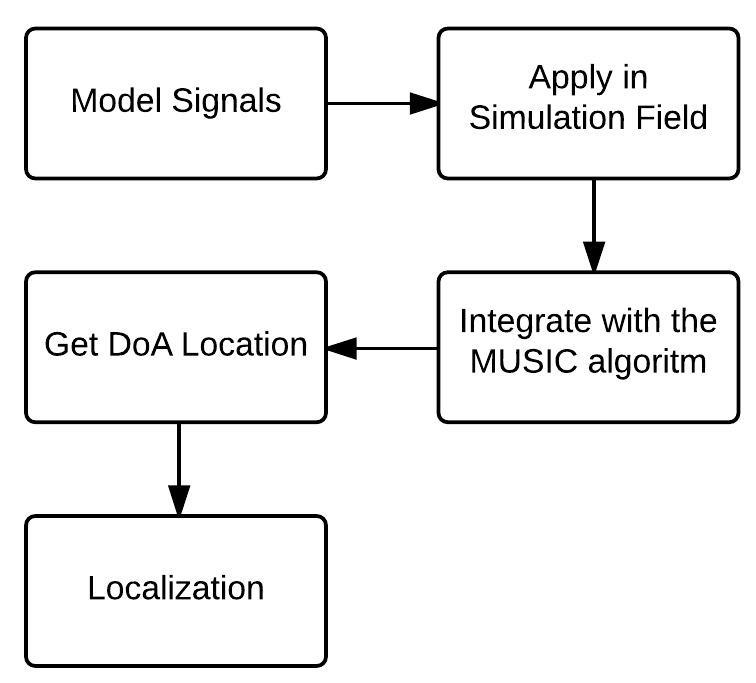
\includegraphics[width=0.4\textwidth]{procedure}
	\caption{Simulation Procedure}
	%\label{fig1}
	\end{figure}
	
In the simulation is designed to see locations of robots and estimated distance by signal strength measured by robot's receivers. The location of the robots and some ranges from the robot are marked. The simulation assumes that field is a 2-D space that ranges 1000 meters by 1000 meters. The robots consist of a transmitter and four receivers with a interval of 0.6 meters. The marked range from robots are 200 meters and 100 meters and 20 meters representing the sensory range and the communication range, the rejection range respectively.



\begin{figure}[ht]
	\centering
	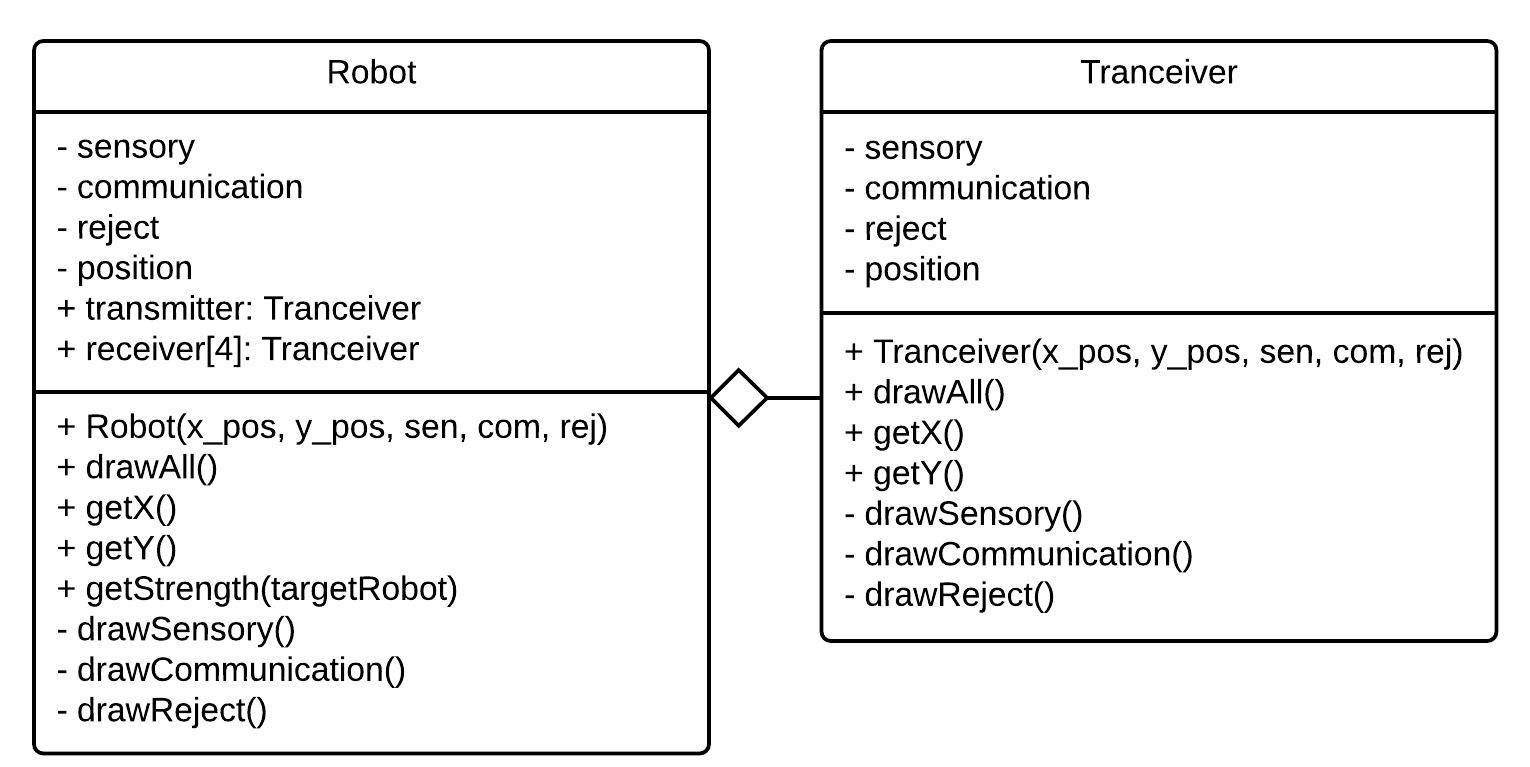
\includegraphics[width=0.4\textwidth]{classDiagram}
	\caption{Class Diagram of the simulation}
	%\label{fig1}
	\end{figure}
	

The simulation is written in MATLAB. The simulation consists of five files: 
\begin{itemize}
	\item simulation.m
	\item Robot.m
	\item Tranceiver.m
	\item simulation.m
	\item getSignalStrength.m
	\item drawCircle.m.
\end{itemize}

The drawCircle.m is used to draw circles on the simulation field to visualize the ranges of robots.

The getSignalStrength.m defines our signal model and accepts a distance value as an argument then returns a value of signal Strength. The model of signal will be discussed later.

Tranceiver.m defines the model of the signal transmitter and receiver using class. This class has four kinds of class member: sensory, communication, reject, and position. The class member sensory, communication, and reject are floating points in meters, representing those name of range. The class member position represents four 

Robot.m defines the class of the robot that has five instances of Tranceiver class:one is for transmitter and the other four is for receiver. This class has a method getStrength() that takes another instance of Robot and calculate signal strength between two robots. 

\subsection{Formula}
The equation of path loss is:
\begin{equation}
L(d)=10*n*log_{10}d + C
\end{equation}
where $L$ is the path loss in decibels, $n$ is the path loss exponent, $d$ is the distance between the transmitter and the receiver, usually measured in meters, and $C$ is a constant which accounts for system losses.
\par
In our model, we use a reference distance and signal strength to get the signal strength:
\begin{equation}
p_{L}(d)=L(d_{0})-20log_{10}(d/d_{0})
\end{equation}
where $d_{0}$ is the reference distance of an antenna, $L(d_{0})$ is the signal strength at $d_{0}$. The value of $d_{0}$ and $L(d_{0})$ depends on characteristic of an antenna.
\\
\vspace{1cm}

The Gaussian White Noise has the probability density function $p_{G}$ of a normal distribution with random variable $x$ in our case is:
\begin{equation}
p_{G}(x)={\frac {1}{ {\sigma\sqrt {2\pi }}}}e^{-{\frac {x^{2}}{2\sigma}}}
\end{equation}
where $\sigma$  the standard deviation. The standard deviation in our model depends on performance of antenna, which can be represented as Signal-to-Noise Ratio (SNR).
\vspace{1cm}

The Rayleigh fading is the effect when there are objects like wall in the field that scatter the radio signal. The Rayleigh fading has a model with Rayleigh distributed probability density function, that is:
\begin{equation}
p_{R}(r)={\frac {2r}{\Omega }}e^{-r^{2}/\Omega },\ r\geq {}0
\end{equation}
where $R$ is random variable, and $\Omega$ is the mean value of square of $r$: $\Omega = E(R^{2})$.
\vspace{1cm}

To sum up, the received signal strength of the receiver antenna is:
\begin{equation}
p(d)=p_{L}(d)+p_{G}(x)+p_{R}(r)
\end{equation}
where $L(d)$ is the path loss, $p_{G}(x)$ is the Gaussian White Noise, and $p_{R}(r)$ is the Rayleigh fading.
\vspace{1cm}


The frequency estimation function for MUSIC is:
\begin{equation}
\hat P_{MU}(e^{j \omega}) = \frac{1}{\sum_{i=p+1}^{M} |\mathbf{e}^{H} \mathbf{v}_i|^2},
\end{equation}
where $\mathbf{v}_i$ are the noise eigenvectors and
\begin{equation}
\mathbf{e} = \begin{bmatrix}1 & e^{j \omega} & e^{j 2 \omega} & \cdots & e^{j (M-1) \omega}\end{bmatrix}^T.
\end{equation}
%\begin{figure}[h]
%\centering
%\includegraphics[width=0.8\linewidth]{img/img1}
%\caption{3D terrain surface}
%\label{fig4}
%\end{figure} 

\section{Evaluation}
\label{sec:evaluation}
\section{Simulation Result}
\indent 
	We use simple version of signal modelling only considering path loss with some noise signal. 
\par 
	The following graphs are 4 simulation results that randomly allocate 4 robot objects and one signal power vs. distance simulation figure :\\
 
\begin{figure}[h]
\begin{minipage}[h]{0.4\linewidth}
	\centering
	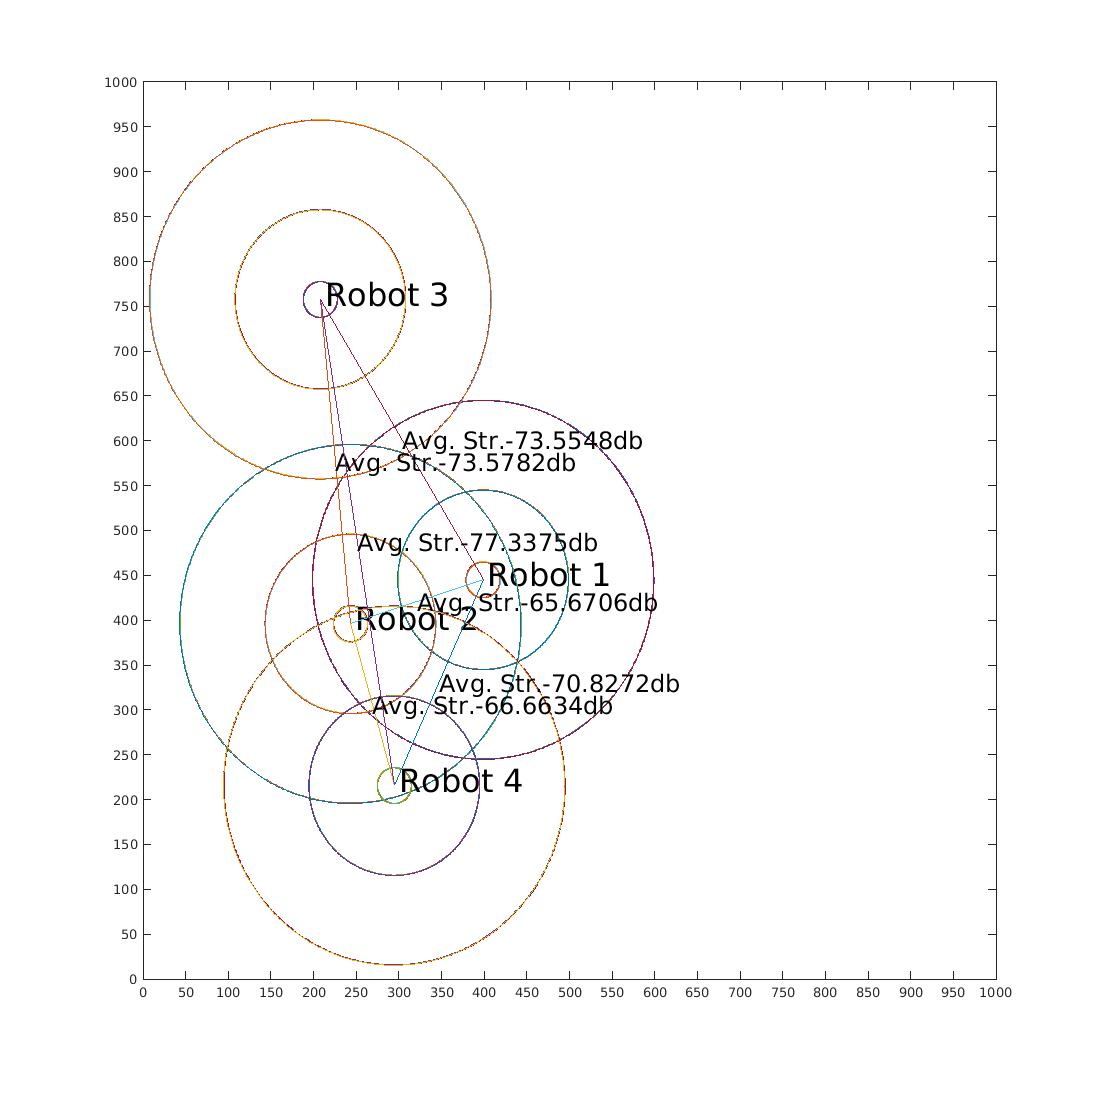
\includegraphics[width=\textwidth]{simulation1}
	\end{minipage}
	
	\begin{minipage}[h]{0.4\linewidth}
	\centering
	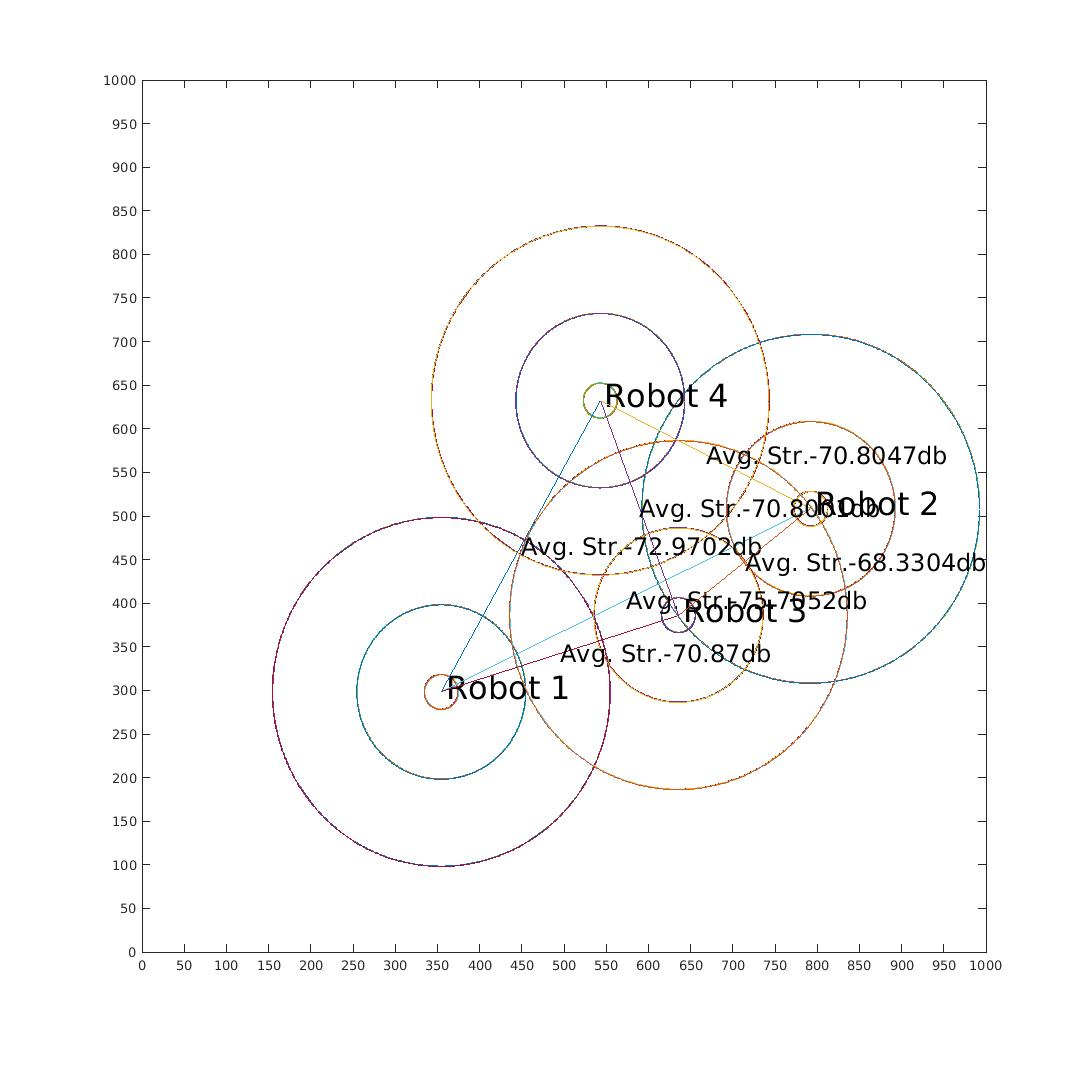
\includegraphics[width=\textwidth]{simulation2}
	\end{minipage}

	\begin{minipage}[h]{0.4\linewidth}
	\centering
	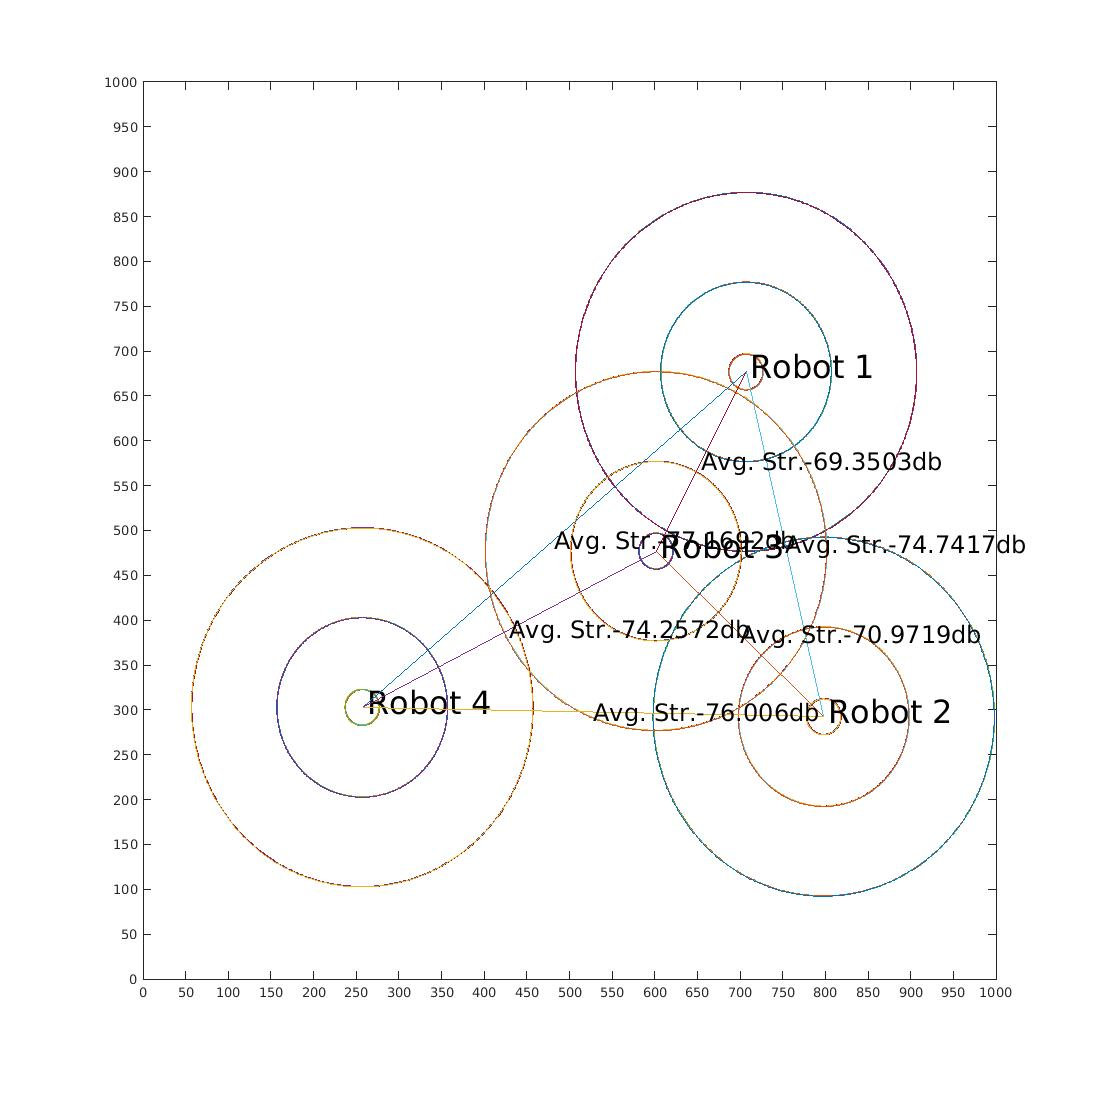
\includegraphics[width=\textwidth]{simulation3}
	\end{minipage}
	
	\begin{minipage}[h]{0.4\linewidth}
	\centering
	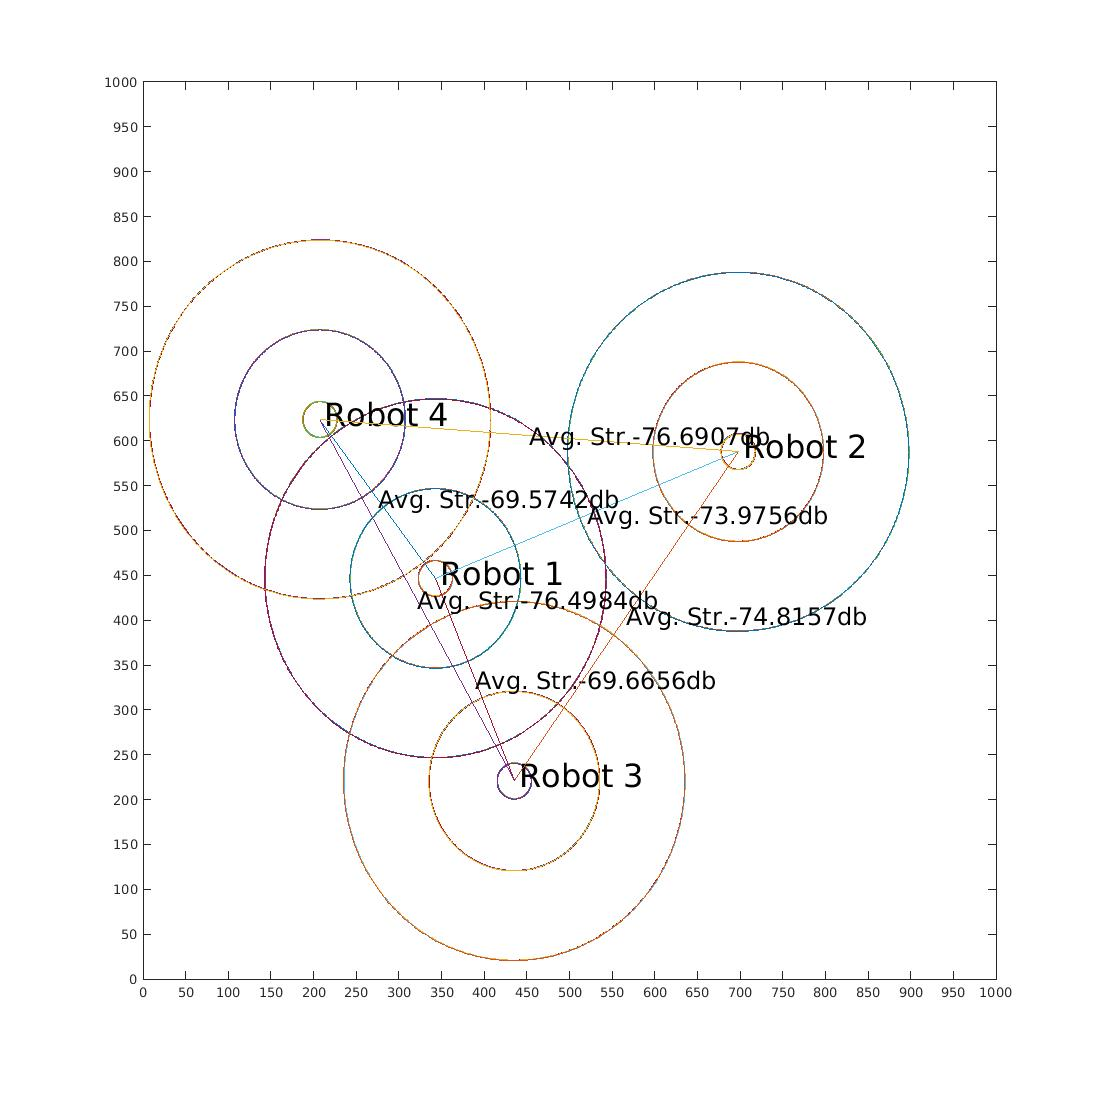
\includegraphics[width=\textwidth]{simulation4}
	\end{minipage}

\caption{Four sample simulations}

\begin{minipage}[h]{\linewidth}
	\centering
	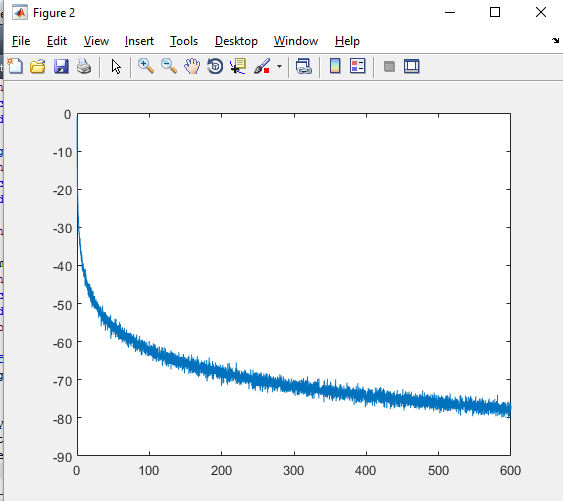
\includegraphics[width=\textwidth]{simulation5}
	\end{minipage}
	\caption{Power vs. Distance}
	
\label{fig:image2}
\end{figure}



\section{Conclusion}




 
%\cite{temp}
%\cite{introtemp} 
%\cite{introccd} 
%\cite{sensortech}
%\cite{Sensor2003}
%\cite{Sensors}
%\cite{Rindner1969}
%\cite{Information2015}


% trigger a \newpage just before the given reference
% number - used to balance the columns on the last page
% adjust value as needed - may need to be readjusted if
% the document is modified later
%\IEEEtriggeratref{8}
% The "triggered" command can be changed if desired:
%\IEEEtriggercmd{\enlargethispage{-5in}}

% references section

% can use a bibliography generated by BibTeX as a .bbl file
% BibTeX documentation can be easily obtained at:
% http://www.ctan.org/tex-archive/biblio/bibtex/contrib/doc/
% The IEEEtran BibTeX style support page is at:
% http://www.michaelshell.org/tex/ieeetran/bibtex/
%\bibliographystyle{IEEEtran}
% argument is your BibTeX string definitions and bibliography database(s)
%\bibliography{IEEEabrv,../bib/paper}
%
% <OR> manually copy in the resultant .bbl file
% set second argument of \begin to the number of references
% (used to reserve space for the reference number labels box)
%\begin{thebibliography}{1}
%\bibliographystyle{abbrv}

%\bibitem{IEEEhowto:kopka}
%\bibliographystyle{IEEEbib}
\bibliographystyle{unsrt}
%\bibliography{IEEEabrv,bare_conf}

\bibliography{bare_conf.bib}
%H.~Kopka and P.~W. Daly, \emph{A Guide to \LaTeX}, 3rd~ed.\hskip 1em plus
%  0.5em minus 0.4em\relax Harlow, England: Addison-Wesley, 1999.

%\end{thebibliography}




% that's all folks
\end{document}


